
\documentclass[12pt, titlepage]{scrartcl}
\setkomafont{disposition}{\normalfont\bfseries}

\title{\textbf{\textit{Astrea}} Constellation }
\subtitle{Project Charter \vspace{7cm}}


%\author{ Pol Fontanes Molina, \and  Victor Martinez Viol, \and David Morata Carranza,
%        Josep Maria Serra Moncunill, \and
%        Eva Mar\'{i}a Urbano Gonz\'{a}lez,  \and
%        Nando Herr\'{a}n Albelda, \and
%        Lluís Foreman Campins, \and
%        Oscar Fuentes Mu\~noz, \and
%        Silvia Gonz\'{a}lez Garc\'{i}a, \and
%        Laura Pla Olea, \and
%        Joan Cebrian,  \and
%        Josep Puig Ruiz, \and
%        Roger Fraixedas	, \and
%        Marina Pons, \and
%		Sergi Tarroc, \and
%		Xavi Ti\'{o}, \and
%		Boyan Naydenov
%}
\author{\emph{Group 4}}

\date{\textit{\today}}

\usepackage{blindtext}
\usepackage[utf8]{inputenc}
\usepackage{fancyhdr}
\usepackage{lastpage}
\usepackage{booktabs}
\usepackage{pdfpages}
\pagestyle{fancy}

\lhead{\textit{Astrea}}
\chead{}
\rhead{ESEIAAT
Engineering Projects Department}
\lfoot{}
\cfoot{ \thepage \hspace{1pt}/\pageref{LastPage}}
\rfoot{}


\begin{document}
\maketitle
\tableofcontents
\pagebreak
\pagebreak


\section{Aim of the project}
Design of a \textbf{satellite constellation} dedicated to  communications relay between LEO Cubesats. 


\section{Scope of the project}
This section establishes the scope of the project.

\begin{itemize}
\item \textit{\textbf{WP2:}} Satellite development. the first step of this work package will
consist on an establishment of the mission requirements that influence
any parameter of the satellite. These requirements include size, weight,
needed antennas, spacecraft subsystems and payload. Based on these
conditions a study of existing CubeSat and NanoSat structures will
be carried out in order to find out the most appropriated. Once the
structure will be selected, an adaptation to the mission requirements
will be achieved if needed. According to spacecraft subsystems, the
design will be in charge of a specialized enterprise that will work strictly
following the requirements talked before.

\item \textit{\textbf{WP3:}} Orbital design. The orbit design will be accomplished according
to the results of several studies such as visibility between satellites
and between satellites and ground stations, collision avoidance, orbital
decay avoidance and stated requirements as global coverage, low earth
orbit, low latency. Also the number of satellites and the number of orbital
planes will be deducted from those studies. It is needed to clarify
if the Earth is the only celestial body that will influence the satellites
or others, for instance, The Moon or Jupiter will also have to be considered.
Another study will be carried out so as to reach a reliable
conclusion about this issue. The specific existing legislation will be
taken into an account and followed during all the orbit development.

\item \textit{\textbf{WP4:}} Launch systems. Concerning to launch systems, a comparison
among the existing launch platforms will be carried out to find
out the one that fulfills the mission requirements and a reasonable economical
conditions. Also, a launching window/s will be reserved if the
launch platform chosen requires it. The recommendations of Corporation
Name will be followed and their application form will be filled
up to ensure all the launch procedure accomplishes the legislation.

\item \textit{\textbf{WP5:}} Operation. An analysis will be done to clarify how many
ground stations must operate and the possibility of placing a central one
in UPC ESEIAAT. A suitable ground station will be selected among
the existing ones. Regarding communication protocols between satellites
of the constellation, external satellites and ground stations, the
1
common protocols used now a days will be adapted to the constellation
needs. An end of life strategy will be designed according to
CubeSat lifespan, orbit decay, replacement stratagem of the company
and legislation procedures.

\item \textit{\textbf{WP6:}} Exhibition. In order to culminate de project, several exhibitions
will be executed. Two of them related to the satellite itself, a
satellite render and a mock-up, and one linked to the overall project
that will consist on a simulation constellation at full service.
2

\end{itemize}

\section{Basic requirements of the project}
\begin{table}[htb]
\centering
\caption{Project Requirements}
\label{my-label}
\begin{tabular}{@{}ll@{}}
\toprule
\textbf{Feature} & \textbf{Description}                                                                                                                                                          \\ \midrule
1                & \begin{tabular}[c]{@{}l@{}}Provide communication relay between two LEO nanosatellites with a \\ latency \textbf{lower than 1 minute}.\end{tabular}\vspace{0.3cm}                                                 \\
2                & \begin{tabular}[c]{@{}l@{}}Provide communication relay between a LEO nanosatellite and the ground \\ with a latency \textbf{lower than 5 minutes.} (Iridium provides Earth Communications \\ with a latency of 1800ms).\end{tabular}\vspace{0.3cm}                                                                                        \\
3                & \begin{tabular}[c]{@{}l@{}}Back-up system prepared to handle \textbf{up to two major failures} in the system.\\ A major failure can be defined as the loss of a client’s satellite coverage.\end{tabular}\vspace{0.3cm}                                                 \\
4                & \begin{tabular}[c]{@{}l@{}}Switch time after failure happens, shall be\textbf{ below 6 hours}.\end{tabular}\vspace{0.3cm}                                                                                                     \\
5                & \begin{tabular}[c]{@{}l@{}}Each Satellite Node volume should be equal or \textbf{lower than a 3U Cubesat.}\end{tabular}\vspace{0.3cm}                                                                                                     \\
6                & \begin{tabular}[c]{@{}l@{}}Each Node should be able to handle \textbf{at least 50 Mbit/s} of data rate.\end{tabular}\vspace{0.3cm}                                                                                                     \\ \bottomrule
\end{tabular}
\end{table}

\section{Justification } \label{justification}
\paragraph{}Nowadays, different universities, research centers and an incresing amount of companies are developing small satellites more and more. These are much more economic and therefore, today’s space access achievability has increased substantially. With that, small satellite constellation missions have been proposed, such as \textbf{QB50} project.

\paragraph{}These complex systems already need to configure and maintain dynamic routes, manage intermediate nodes, and reconfigure themselves to achieve mission objectives. Hence, inter-satellite is both important for satellites that fly in formation and need interconnection, and for single nanosatellites that may require low-latency communication with the ground.


\section{Organization of the group}


\subsection{Hierarchy}
\paragraph{}
Designing a nanosatellite constellation is quite ambitious and requires lots of work because there are many things to consider. In order to build a work strategy, the project is divided in tasks that will be described later on. As the different tasks depend on each other, the project members have decided to follow a hierarchy. Every task is developed by a small team between 2 and 5 people depending on the amount of work the task requires.
\paragraph{}
Each small team has to have a coordinator which has two principal functions. The first one is to manage the group so he is responsible for the good organisation and progression of the task. The second is that he is the voice of the team. That means that the coordinator is the one who represents his work team when transferring information to the other group coordinators and the project managers and vice versa. 
\paragraph{}
Finally over all the teams there is the project manager who maintains order, ensures the project progress and manages people for major decisions. Finally there is also a secretary in charge to write the minutes of each meeting.


\subsection{Documents Organisation}
\paragraph{}
Nowadays, the internet is crucial for teamwork because it provides lots of tools that improve networking such as sharing documents, communicating and even collaborating working. The Astrea team has 17 members so it is essential to define protocol to organise all the documents and information found to take advantage of resources. 
\paragraph{}
The principal communication tool used is \textit{Slack} which is a platform specialised in team communication. \textit{Slack} defines itself as a real-time messaging, achieving and search for modern team which is interesting for us because it allows the group to communicate at all times for punctual doubts and small decisions. For major decisions a date is specified by a \textit{doodle} to meet.
\paragraph{}
Moreover, to share documents we use two platforms: \textit{Slack} and \textit{BSCW}. On \textit{Slack} we put first drafts or documents that can be interesting. \textit{BSCW} is the main information storage because information and documents are stocked and organised in folders.
\paragraph{}
At last, the text editor used to develop the project is Latex which combined with Git allows us to work remotely on a same document without overriding someone else's work. This work system is really interesting for such a big group in order to work on the same document while keeping a record of the changes. 

\section{Planning of the project}

\subsection{Tasks identification from work breakdown structure (WBS)}
%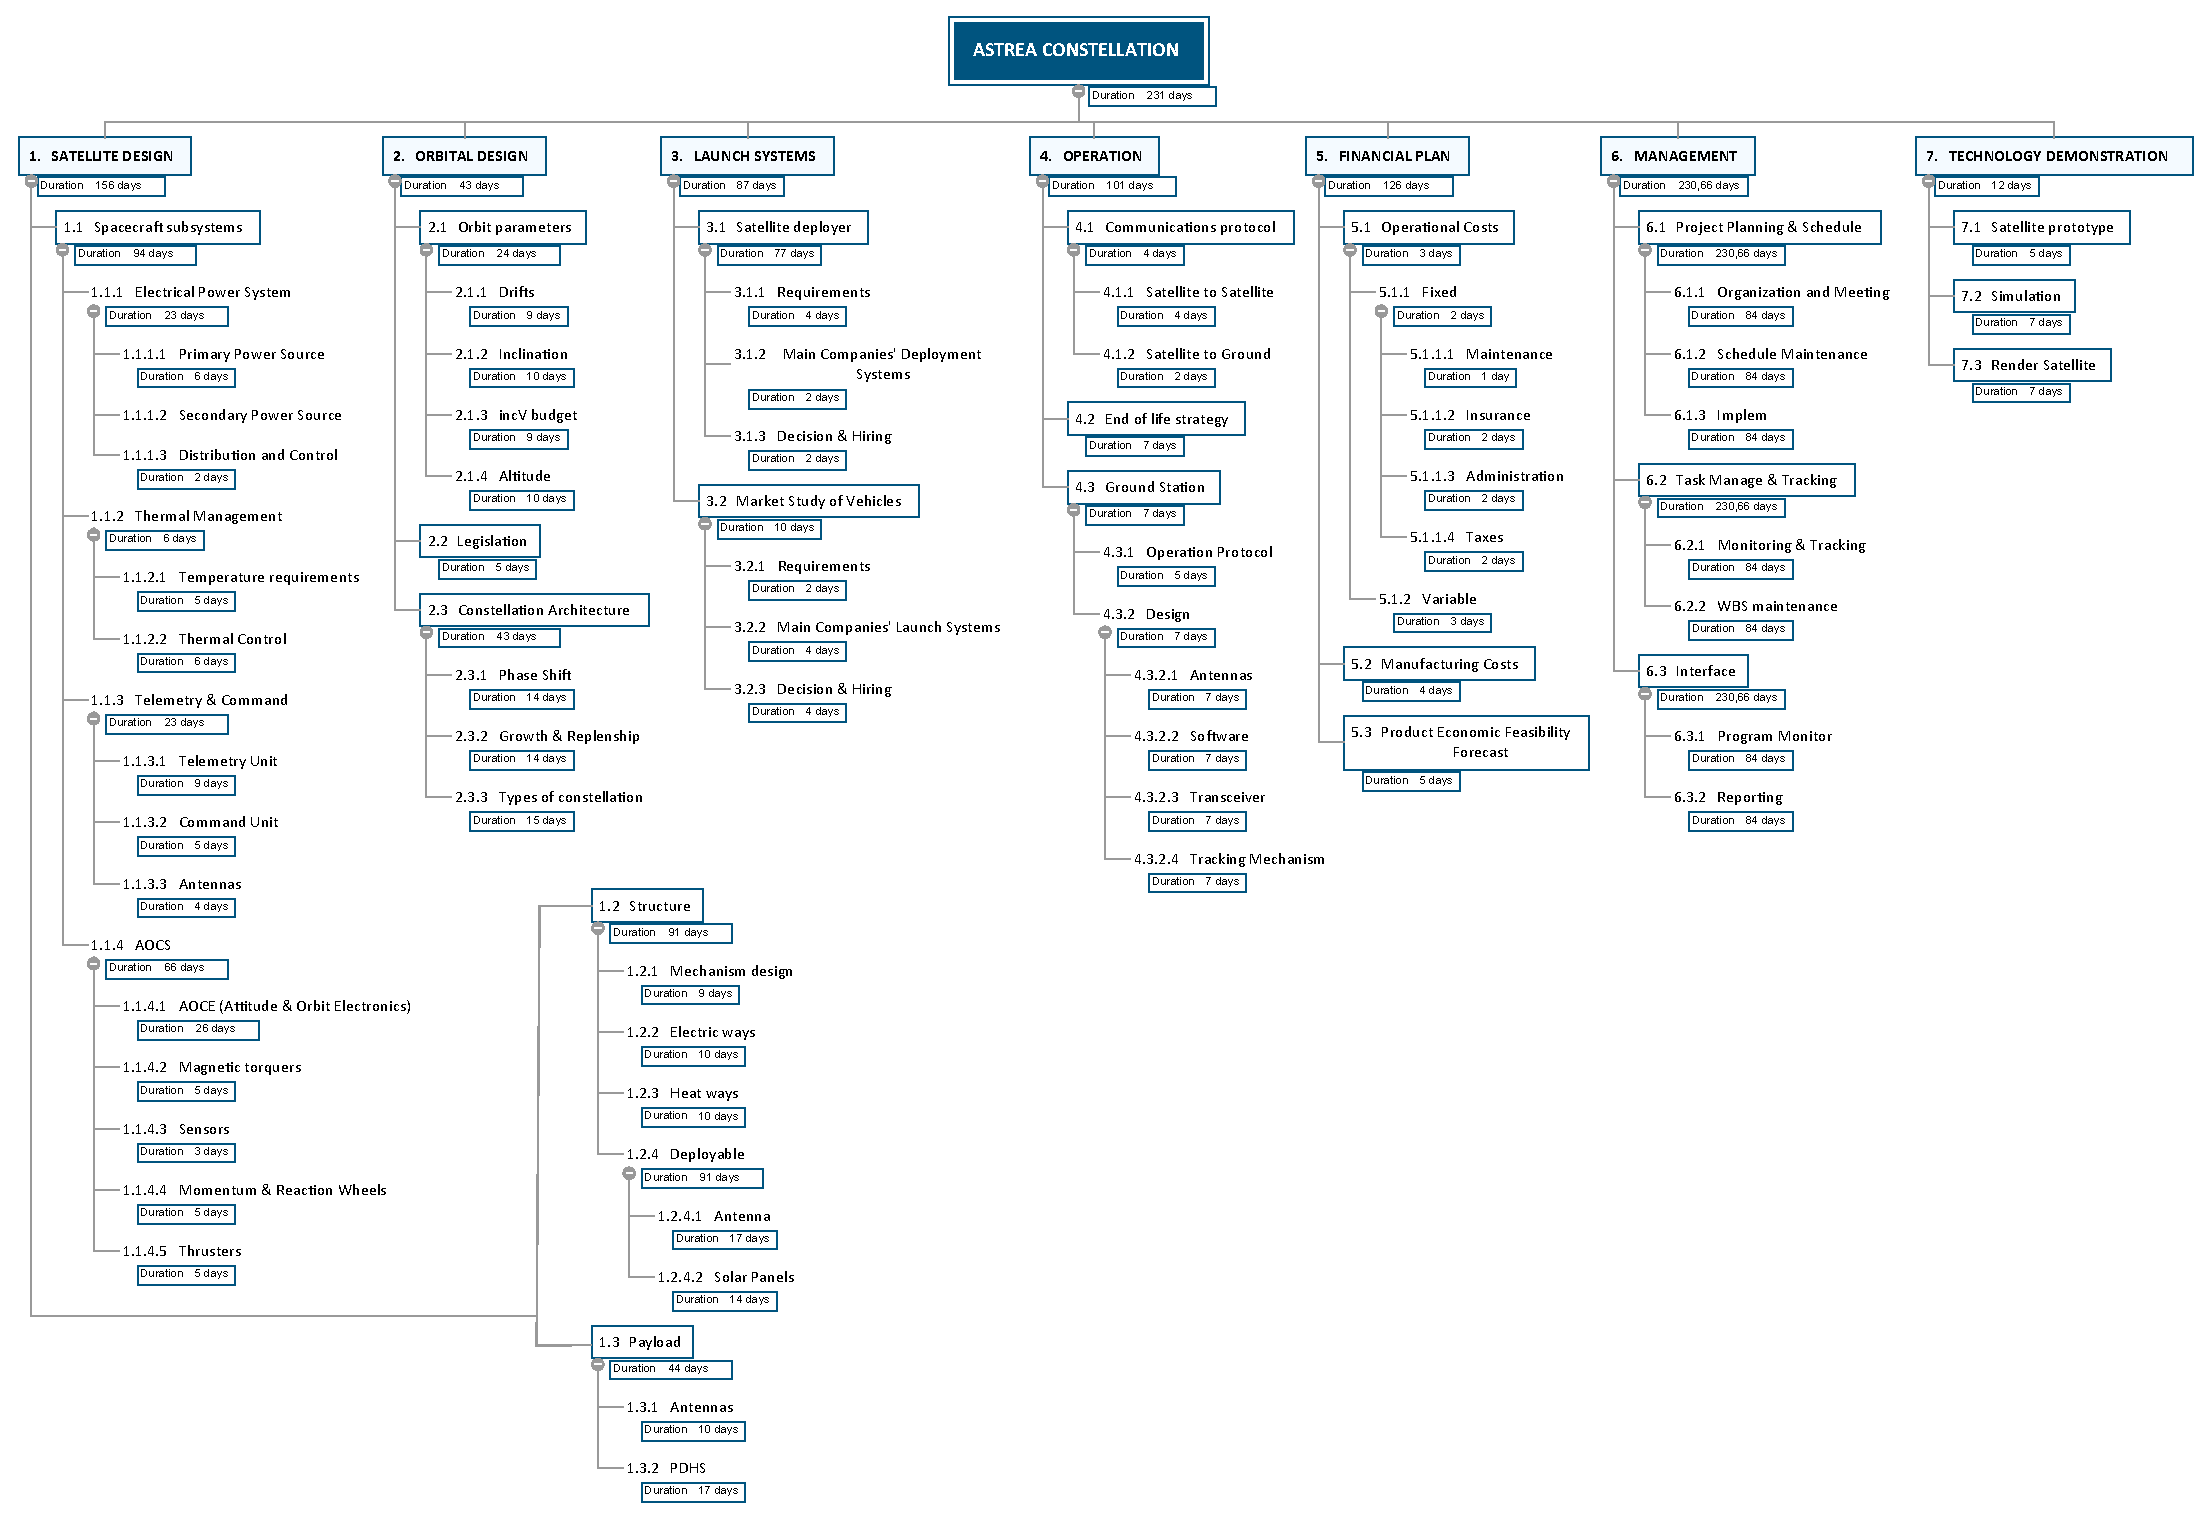
\includepdf[pages={1-}]{./external_pdf/wbs.pdf}

\subsection{Brief tasks description}
\includepdf[pages={1-}]{./parts/pdf/1.pdf}
\includepdf[pages={1-}]{./parts/pdf/2.pdf}
\includepdf[pages={1-}]{./parts/pdf/3.pdf}
\includepdf[pages={1-}]{./parts/pdf/4.pdf}
\includepdf[pages={1-}]{./parts/pdf/5.pdf}
\includepdf[pages={1-}]{./parts/pdf/6.pdf}
\includepdf[pages={1-}]{./parts/pdf/7.pdf}


%\subsection{Interdependency relationship among tasks}
%\includepdf[pages={1-}]{./external_pdf/gantt.pdf}

%\subsection{Human resources and level of effort (hours) to develop each task}
%This is time for all good men to come to the aid of their party!
%
%\paragraph{Outline}
%The remainder of this article is organized as follows.
%Section~\ref{justification} gives account of previous work.
%Our new and exciting results are described in Section~\ref{justification}.
%Finally, Section~\ref{justification} gives the conclusions.


\section{Budget (initial estimation for engineering basic project)}
%\includepdf[pages={1-}]{./external_pdf/budget.pdf}

\pagebreak
%\bibliographystyle{abbrv}
%\bibliography{simple}

\end{document}
